%!TEX root = ../../dissertation.tex
%%%%%%%%%%%%%%%%%%%%%%%%%%%%%%%%%%%%%%%%%%%%%%%%%%%%%%%%%%%%%%%%%%%%%%%%%%%%%%%
\chapter{Introduction}
\label{chap:intro}

%% new thesis stuff
Packet Switching, the process of chunking information into smaller bits, labeling it and transmitting it independently, was first described by Paul Baran in the 1960s~\cite{baran1964distributed}. This changed communication a lot and provided one of the foundations for the emergence of the Internet. 

The original usage intent was mostly limited to remotely logging into and communicating with mainframe computers and transferring files supported by the emergence of new multiuser and multitasking \gls{os}, especially including the release of UNIX in the early seventies.

From these early times countless other services and applications emerged. Today, the Internet is used by hundreds of millions of people and is involved in almost every aspect of daily life. The creation of the World Wide Web --- initiated by Tim Berners-Lee in 1989 --- brought an easily accessible ``user interface'' to the Internet and made adoption for the masses much easier. Today, almost any form of application is available through the Web as a combination of \gls{HTML}, \gls{CSS}, and JavaScript and can be accessed by just opening a Web browser.

But as is the case with many technological fields, the Internet's development was also closely entangled with other advancements. Take the huge Internet music wave beginning in 1999 as an example. It may have been started by the creation of Napster, one of the first peer-to-peer file sharing services. However, without the large improvements in audio compression --- the MP3 audio format in this case --- a few years earlier, computers that could handle decompression as well as compression, and increasing Internet access bandwidth (and fixed service fees), this would not have been possible. 

Similarly, video streaming and sharing sites like YouTube could not have existed without a wide spread availability of digital camcorders and other devices with recording capability, good video compression codes, and an even further increase in access bandwidths. For every advance in access bandwidth new services sprung to life fueling the users' demand for further capacity increases. 

One of the driving factors in this rapid adoption of the Internet and the Web is its content agnosticism, i.e., that no assumptions are made on the transported data. The original idea is to treat every packet and participating node the same and not make any assumptions on specific applications. This provides a level playing field for every contender wanting to offer services. A further concept, called ``End-to-End Principle'', was originally stated as:

\begin{quote}
``The function in question can completely and correctly be implemented only with the knowledge and help of the application standing at the endpoints of the communications system. Therefore, providing that questioned function as a feature of the communication system itself is not possible. [\ldots]''~\cite{saltzer1984end2end}
\end{quote}

This means that any functionality, for example services or applications, or traffic differentiation should only be implemented at the two endpoints of a transmission and not inside the network. Tuning the network to specific applications and implementing functions inside the network, will always only be valid for existing and narrow use cases and could hamper any future future development.

During the past decades these principles have often been discussed~\cite{bhattacharjee1997active, blumenthal2001rethinking, isenberg1997rise, lemley2000end} but are mostly still being upheld in the current Internet topology. Interestingly, this is contrasted by the way \gls{CS} public telephone networks but also mobile networks operate. Here, much effort and intelligence is put into the network, which enables only a very specific set of services, determined solely by the operator, to work, albeit with a relatively high quality.


%%%%%%%%%%%%%%%%%%%%%%%%%%%%%%%%%%%%%%%%%%%%%%%%%%%%%%%%%%%%%%%%%%%%%%%%%%%%%%%%
\section{Video and the Internet}

\begin{figure}[htb]
    \centering
    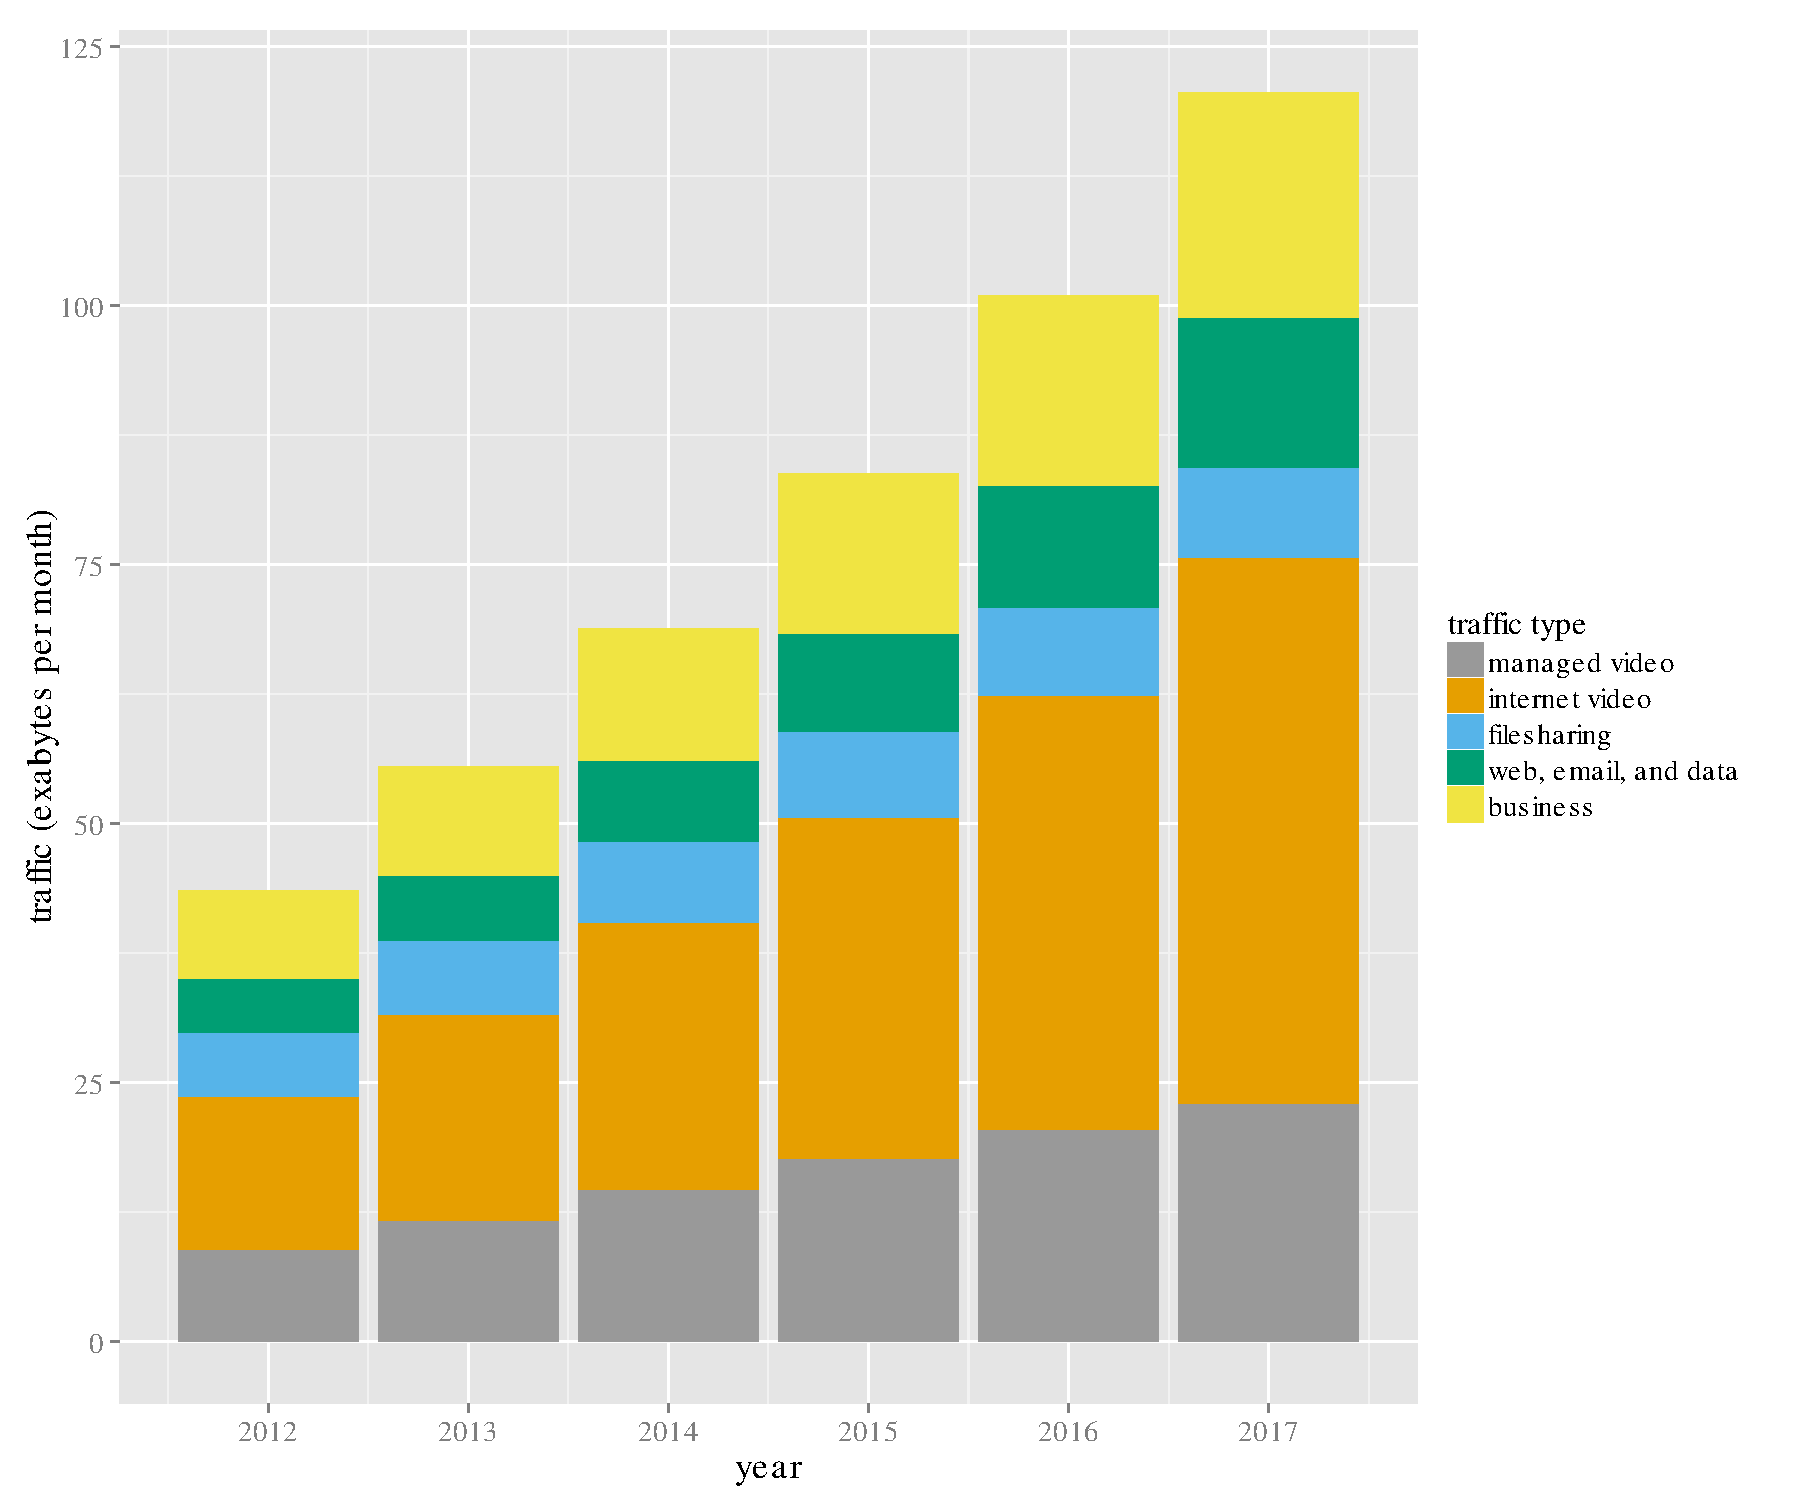
\includegraphics[width=0.9\textwidth]{images/r-cisco-vni-2013.pdf}
    \caption{Cisco's global consumer Internet traffic prediction (data source: \cite{cisco2013VNI}).}
\label{c1:fig:traffic-cisco}
\end{figure}

The total volume of Internet traffic has been rising exponentially for many years as many traffic studies suggest, for example in a Cisco study of ``consumer'' traffic in Figure~\ref{c1:fig:traffic-cisco}. One of the largest contributing factors to today's traffic composition is arguably video traffic. It can be most dominantly observed in the mix of North America's fixed access depicted in Figure~\ref{c1:fig:traffic-netvine-fixed}. The two main sources for this video traffic are typically streaming services like YouTube\footnote{\url{https://www.youtube.com}} and Netflix\footnote{\url{https://www.netflix.com}}, or live streaming and casting sites like Twitch\footnote{\url{http://twitch.tv}}. 

\begin{figure}[htb]
    \centering
    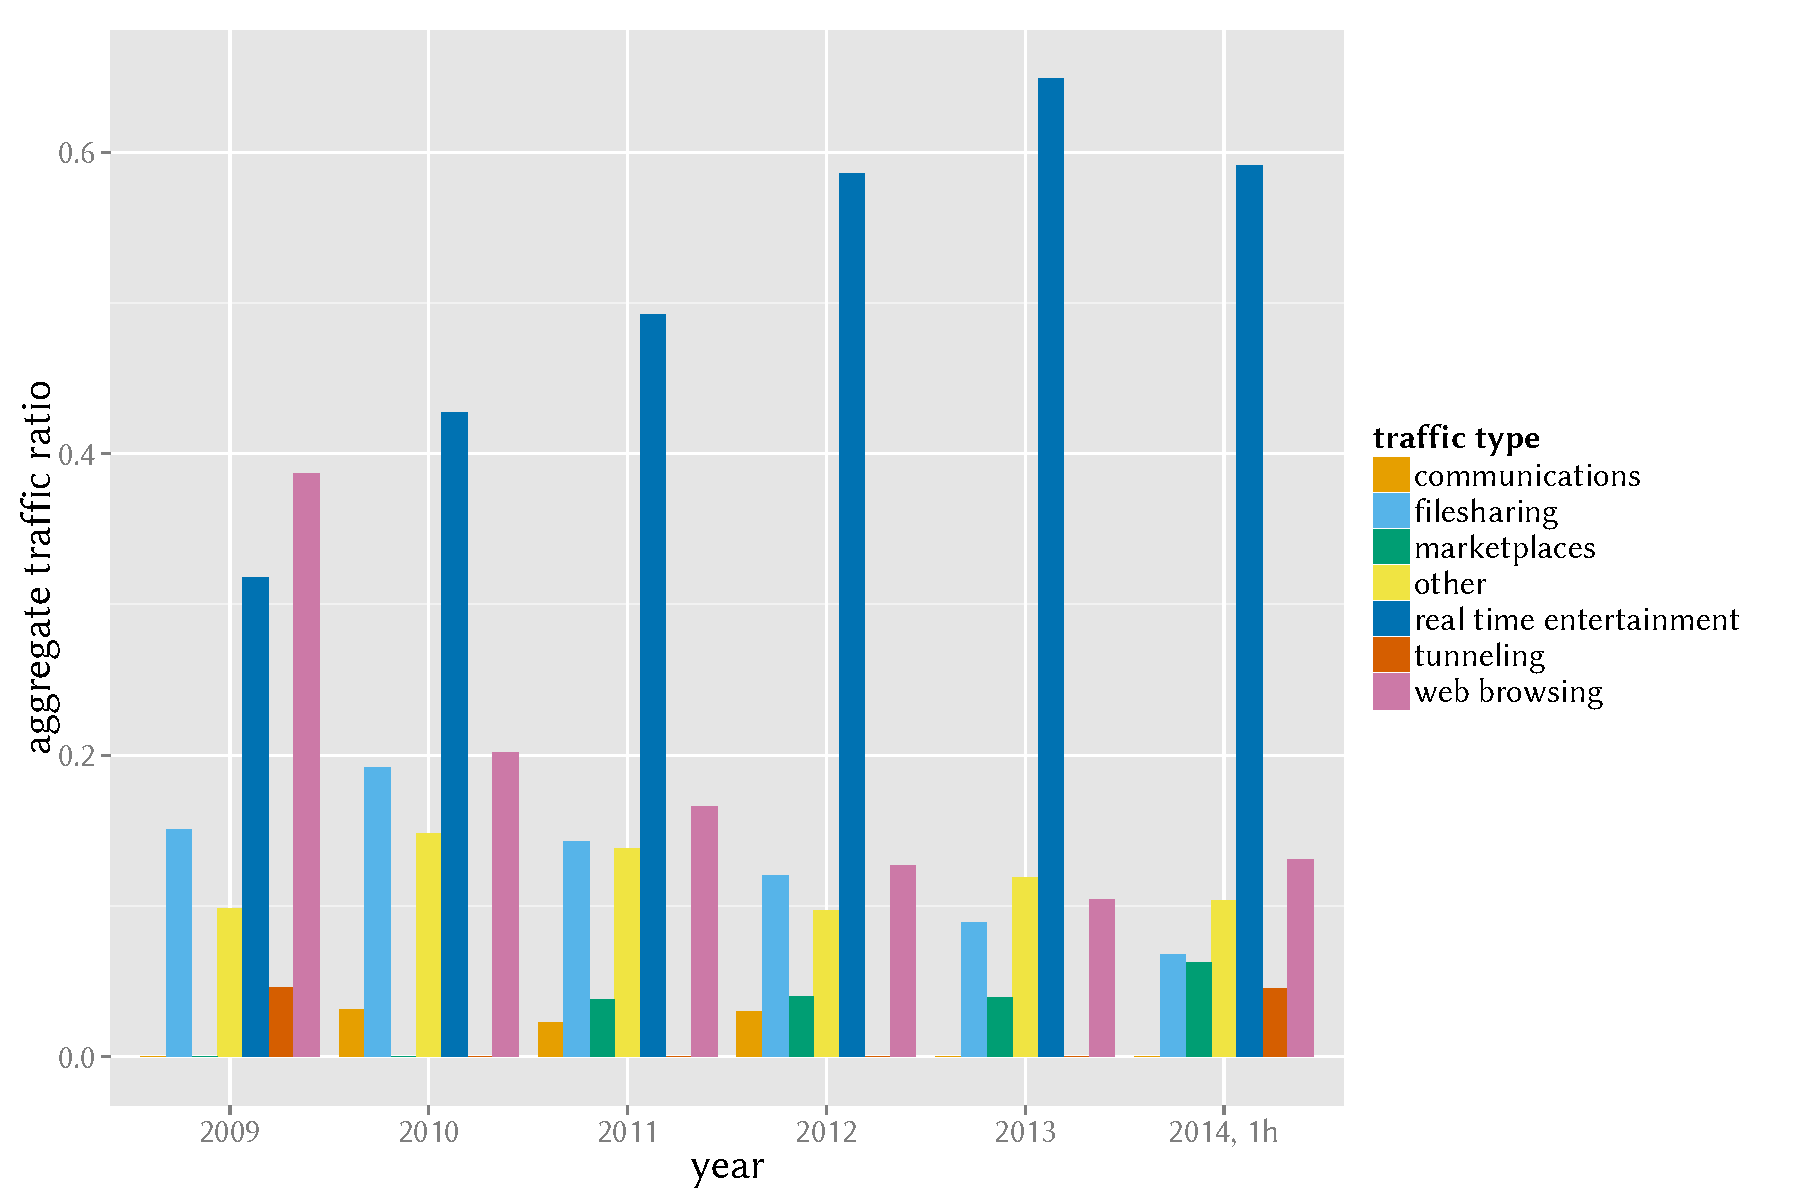
\includegraphics[width=0.9\textwidth]{images/r-netvine-phenomena-fixed.pdf}
    \caption{Traffic composition of North American peak fixed access aggregate traffic (data source: \cite{sandvine_internetphenomena}.} %\cite{sandvine_spring2013}).
\label{c1:fig:traffic-netvine-fixed}
\end{figure}

Studies predicting the development of the Internet's traffic also tell of the large influence of video traffic in the near future. As the video traffic volume has become so predominant, it is very important to understand its dynamics from a modeling and performance evaluation point of view, as specific behaviors of video traffic might significantly influence the underlying network and vice versa. 

Protocols specifically created for the purpose of video streaming --- defined as ``watching the video while it's still being transmitted'' --- have existed for a long time and their behavior is well researched. The most prominent is \gls{rtp}, which has been specified as early as 1996~\cite{rfc1889}. And yet they are not responsible for the gross of the Internet's video traffic seen today.

Instead, a new class of \gls{TCP}-based and not standardized streaming approaches has arisen, which integrate themselves much better into the current Web ecosystem. And they are using completely different modes of transportation and control. Finding ways to investigate these new streaming protocols, including their categorization, measurement, and modeling, will be the first task of this thesis.

Streaming, and media transport in general, is also not just relevant for the purpose of watching videos, there are many more fields of use with similar requirements. For example, so-called ``cloud gaming'' applications have become more popular in recent years. Here, video games are run on large virtualization clusters with the input and video output being streamed from and to the actual game client, putting a huge emphasis on achieving low latency. Refer to, e.g., \cite{4795441}, \cite{wang2009modeling}, \cite{jarschel2011cloudevaluation}, or \cite{ct2010wolken} for further information on this topic.


%%%%%%%%%%%%%%%%%%%%%%%%%%%%%%%%%%%%%%%%%%%%%%%%%%%%%%%%%%%%%%%%%%%%%%%%%%%%%%%%
\section{The Mobile Network Below}

Much of today's Web interactions are today carried out over mobile networks using smartphones. Despite their rapid evolution, mobile networks still carry much heritage from their circuit switching roots.\footnote{For an historical overview of mobile phone standards refer to \url{https://en.wikipedia.org/wiki/History_of_mobile_phones}.}
Starting in the 1950s with early analog predecessors like the German ``A-Netz'' and first generation cellular structured networks in the eighties, mobile telephony entered the fully digital world with the European \gls{GSM} and competing \gls{CDMA}-based technologies around the year 1991. This was similar to the development in the \gls{POTS} with its shift away from the analog roots to digital circuit switching technologies like \gls{ISDN}.

Because of the huge success of \gls{GSM} and its packet-switching extension \gls{GPRS} it was used as a blueprint for the following mobile network standard evolutions \gls{UMTS} (including \gls{HSPA} and \gls{HSPA+}), \gls{LTE} and also the upcoming \gls{LTE} Advanced. 

Through this heritage, many mobile network elements and protocol have undergone only minor changes since their \gls{GSM} versions. Due to the hereditary roots in \gls{CS} networks \gls{CS}, a large amount of state is kept inside the network a explicitly managed through a high volume of signaling interactions. This can create a wide range of problems, creating unwanted interactions of specific traffic patterns with the control plane and overwhelming the network's control plane structures. 

\begin{figure}[htb]
    \centering
    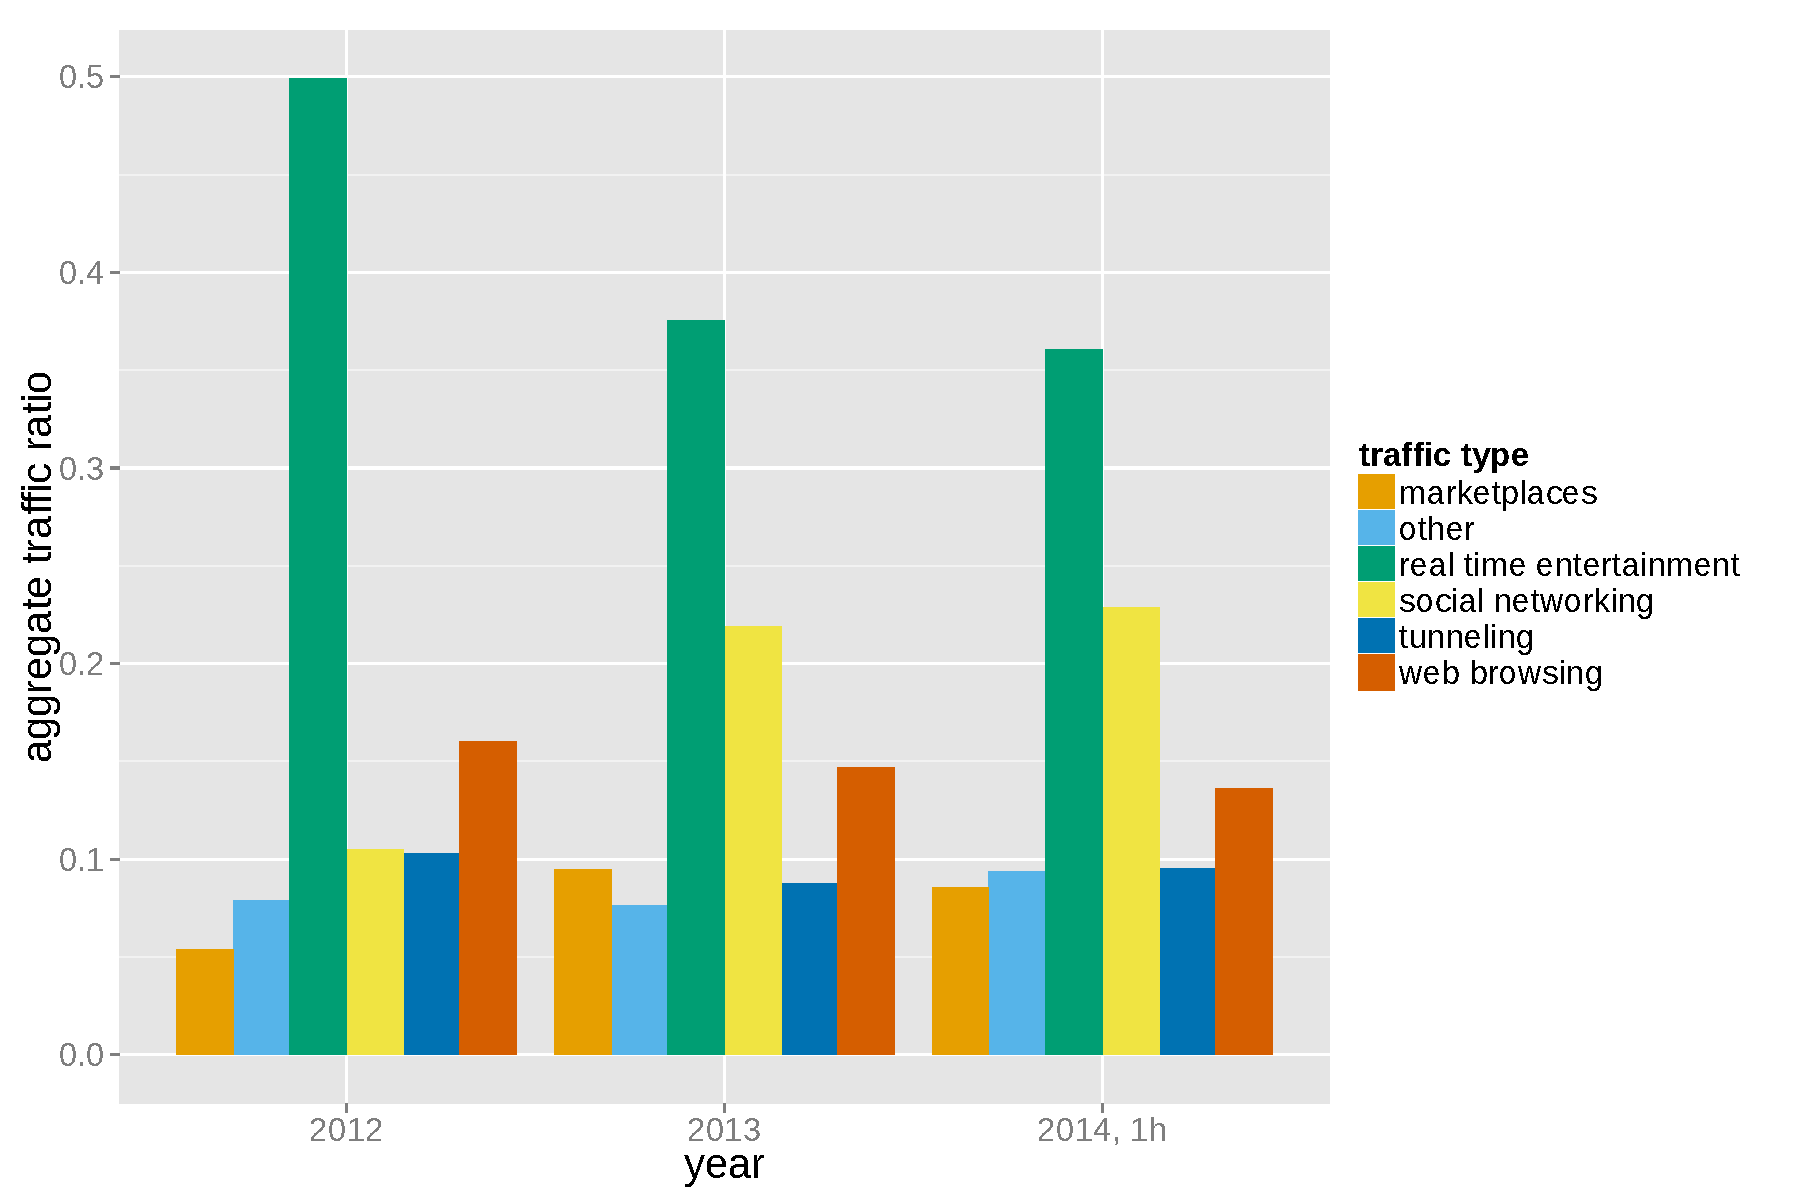
\includegraphics[width=0.9\textwidth]{images/r-netvine-phenomena-mobile.pdf}
    \caption{Traffic composition of North American peak mobile access aggregate traffic (data source: \cite{sandvine_internetphenomena}.} %\cite{sandvine_spring2013}).
\label{c1:fig:traffic-netvine-mobile}
\end{figure}

These issues have only begun to show up in recent years due to the large influx of new user and usage scenarios. Traffic in cellular networks follows a development similar to that of the Internet as a whole. Through the advent of affordable high performance smartphones, a thriving mobile application ecosystems, and faster access technologies many are now using their phones as the primary device for interacting with the Internet. Video, too, has here become one of the largest contributors of cellular traffic as Figure~\ref{c1:fig:traffic-netvine-mobile} depicts.

However, heavy traffic on a stateful network poses unique challenges to the performance, the architectural design, and dimensioning of network protocols. This becomes even more pronounced by the circumstance, that operators and vendors usually regard any details on mobile networks equipment as closely kept trade secrets Thus, little is known of the exact make-up of these networks as they are closely guarded secrets of the operator.

The investigation of the signaling structures in the core of today's mobile networks represents the second task of this thesis. It is also closely interlocked with the evaluation of video streaming traffic as they are nowadays often seen together.


%%%%%%%%%%%%%%%%%%%%%%%%%%%%%%%%%%%%%%%%%%%%%%%%%%%%%%%%%%%%%%%%%%%%%%%%%%%%%%%%
\section{Research Methods and Approaches}

As is the case with any scientific endeavor, this work is based on a specific set of tools and knowledge of many years of prior research. Measuring, evaluating and modeling is standard practice in many fields. Therefore, tools are available to tackle any kind of problem, but one still has to choose the most fitting ones for a given specific issue.

\begin{figure}[htb]
    \centering
    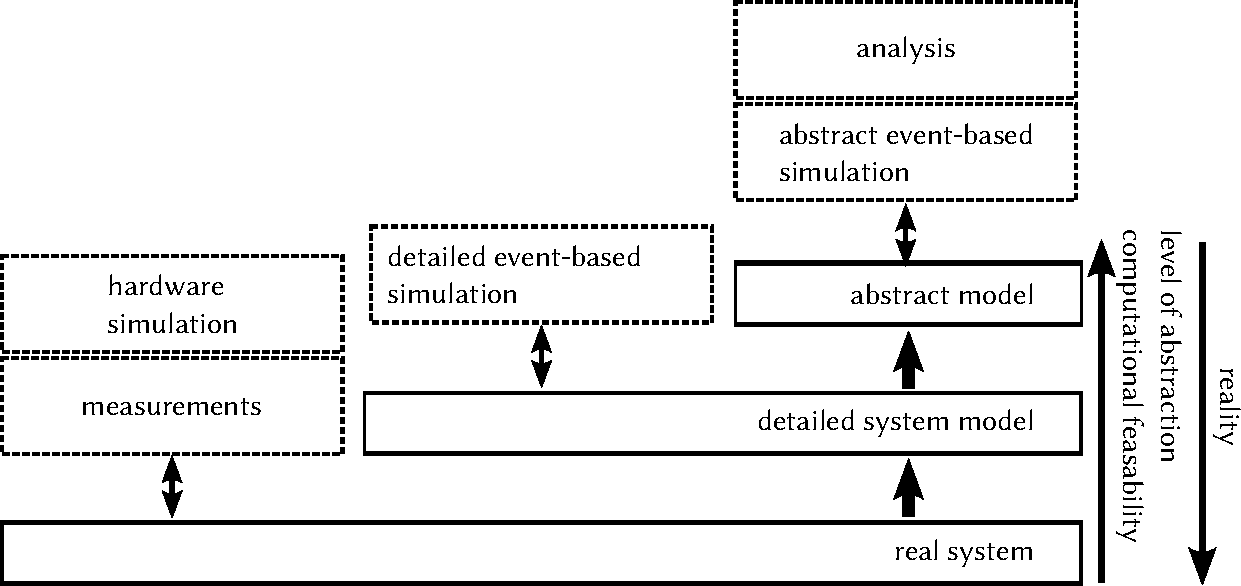
\includegraphics[width=1.0\textwidth]{images/apparatus.pdf}
    \caption{Methodical solution spaces and apparatus comparison.}
\label{c1:fig:appcomp}
\end{figure}

Figure~\ref{c1:fig:appcomp} attempts to categorize all tools available to a performance analyst, with their corresponding level of detail and abstraction.

The most precise results will always be achieved through actual measurements of the actual system under scrutiny. This will give a point of reference and can be used to validate the accuracy of other methods. But it also comes with a hefty price of huge amounts of data to process and understand. With such measurements at hand, one can now start to make sense of this data and extract the relevant features observed in this process.

Aside from measurements on implementations there are three further possible approaches to widen the scope: emulation, simulation, and mathematical analysis or analytical models. An emulation tries to resemble implemented functionality as closely as possible with the cost of high complexity. While there are many forms of emulation, most relevant to this type of research is the network emulator. Instead of having a real network, parts of it are substituted with emulating hardware or software that alters the \gls{QoS} parameters of transmissions. But emulations always just replace parts of the actual system and therefore its capability to scale is limited.

This is where simulations come into play, implementing all internal and external functionality, including the physical nodes and the network in software. A typical \gls{DES} can have subtle functional differences but can be scaled almost boundless, limited only by the available processing time. 

Prior to any simulation or emulation and following every measurement on a system is of course the mathematical analysis of existing data. Through this models are built abstracting the system the data is gathered from. With every iteration the model can be refined and new hypotheses formed.
A mathematical analysis, for example using queuing theory and stochastic models, can then further broaden the understanding of the system. A proper queuing theory model can already give great insights into the load dynamics of the modeled system and serve as a tool in future planning processes.


%%%%%%%%%%%%%%%%%%%%%%%%%%%%%%%%%%%%%%%%%%%%%%%%%%%%%%%%%%%%%%%%%%%%%%%%%%%%%%%%
\section{Research Contributions}

With the increasing prevalence of video streaming in mobile networks, it is important to understand the relationship and interworking between these two. To achieve this with the discussed tools at hand the topic will be separated into two standalone lines of research discussing video streaming on the one hand and mobile networks on the other. Only after the individual issues have been thoroughly investigated on their own the efforts are merged again and actual video streaming in mobile networks is explored.

The first line will be an investigation of current video streaming mechanisms and services facilitating them. All of the investigated streaming protocols are comparatively young and similar. Protocol is put in quotation marks for a reason here. Many of the approaches are not protocols in the classical sense. They do not follow a specification of any standards body, be it \gls{ISO}, \gls{ITU} or the \gls{IETF}. 

Also, their main distinction does lie in the usage of the network and the video transport due to the reliance on typical Web protocols. Rather, much of the differences stems from the behavior of the actual application. Specifically, the way data is requested and retrieved and the video displayed, including its reaction to undesirable circumstances, e.g., having insufficient data in the playback buffer. Surprisingly, even just with these simple rules, applications can easily distinguish themselves from one another. Making the correct decisions to events can greatly influence the quality of the video playback. 

During the investigation a model will be created that describes all the common elements in the streaming process. This model and additional knowledge of the structure and similarities of the applications enables further, more complex research efforts. For example, through a performance analysis streaming protocols can be compared to each other. Or interrelations to the network's transport layer and other influences of the network on streaming could be uncovered. 

This especially refers to influences of mobile networks, where many assumptions targeted at wired networks do not hold anymore. One quick example is the circumstance, that the mobile network stack typically conceals any packet loss from its users. Loss will therefore only be experienced as  intermittent times of extremely high latency, which can go as high as several seconds and preventing transport protocols from correctly determining the link conditions and causes erroneous scaling.
This leads to the question, on which kind of information from the network a streaming application could and should depend, or even if there are any actual requirements for streaming.

Gathering this kind of information can result in a better understanding of the quantitative attributes related to these new forms of streaming. The results can be used as an analytical and testing tool for improving the protocols or even lead to different approaches. Furthermore, the thesis aims to provide methods for helping all parties involved in media streaming decide which protocols and methods to choose and which are best suited for specific scenarios.


The second line of research will deal mostly with the control plane of mobile core networks. Using architectural knowledge, collected from the large stack of mobile network specifications, a measurement dataset from an actual core network is evaluated on the basis of its signaling load. Through further statistical analysis of specific signaling interactions a queuing theoretic load model of the core network well be created, abstractly describing the control plane. 

This allows to draw interesting conclusions regarding the load state and its relationship to external influence factors, e.g., to user traffic, in these cellular nets. Building on top of this basis, an alternate model will be introduced that is better able to scale the load than the standard model. These efforts will ultimately help to improve the planning and dimensioning of networks, or even influence future specification iterations to reduce their adherence on signaling.


The third and final topic bridges both of the previous lines. The complete video streaming mobile network stack is re-investigated on a quest for potential sources of influence that impact the quality of the resulting streaming endeavors. The search is made more difficult by the circumstance that the stack is changing rapidly, with protocols being replaced or significantly altered. Examples for this will be given. Ultimately, an approach to reduce the stack's undesired influences will also be discussed in the form of cross-layer information flow.

Evaluating mobile networks and the complete streaming stack is a complex effort, with a vast number of variables to control and keep track of. To give an example, think of the mobility patterns of mobile devices, the resulting handover procedures between cells and the effect on a video stream running during these events. 

In this work, two methods are tackled that deal with this situation. The first method enables one to conduct active measurements on mobile devices while combining them with the metadata from the device's stack and sensors. To achieve meaningful measurement results, the device's state needs to be recorded as precisely as possible. Today's mobile phone have a multitude of sensors and information sources available, which can be exploited here.

The knowledge attained from these previous approaches can then finally be put into a mobile network streaming simulation, which can be more easily scaled up than an active measurement campaign. Through this method, new streaming strategies can be tried out and tested as well as tuned to influences of the mobile network environment.


%%%%%%%%%%%%%%%%%%%%%%%%%%%%%%%%%%%%%%%%%%%%%%%%%%%%%%%%%%%%%%%%%%%%%%%%%%%%%%%%
\section{Structure}

Following these research lines, several contributions are made, which will be broken down into four major chapters.

To introduce to the video streaming investigations, covered in Chapter~\ref{chap:streaming}, at first the protocols and techniques, that have been used in the past, will be described in Section~\ref{c3:sec:background}. This then leads to a broad survey of current protocols. A subset of them will serve as the basis for the presented reliable streaming model. 

Furthermore, to be able to derive \gls{QoE} information from the model, it is necessary to define an evaluation metric and its building blocks. The building blocks, that can be directly gathered from measurements, will be defined and combined with an overview of existing metrics of which a suitable one will be selected in Section~\ref{c3:sec:modeling}. Now that both metric and model are ready, a measurement study using an emulation approach is conducted in Section~\ref{c3:sec:measurements}, investigating the performance of an actual video streaming service with the help of the model under the influence of varying network conditions.

The facets of mobile core networks are put under scrutiny in Chapter~\ref{chap:mobilenets}. As the amount of specifications as well as architecture, procedure, and protocol details is vast, the mobile core architectural background Section~\ref{c4:sec:3gpparchitecture} attempts to put all the basics together with additional related work in Section~\ref{c4:sec:relwork}.

With this foundation laid out, the actual goal of the investigations will now be defined in Section~\ref{c4:sec:loaddefinition}: a novel definition of load in a mobile network, based on the control plane and not just the user plane. To investigate this load a passive measurement data set is used. Section~\ref{c4:sec:methodology} describes the acquisition of the set and how it should be interpreted. The set is then evaluated for its signaling characteristics in Section~\ref{c4:sec:evaluations} and the data is used to formulate two queuing theoretic load models in Section~\ref{c4:sec:modeling} which are then thoroughly  tested using a queuing simulation in Section~\ref{c4:sec:simulation}. With these models mobile network operators can better dimension and plan their networks according to control plane load and not just to accommodate user traffic.


Chapter~\ref{chap:mobilestreaming} includes the various efforts to screen and understand cross-layer influences with the discussion of current and upcoming protocols in Section~\ref{c5:sec:stack-influences} and a remedy in the form of a cross-layer hinting framework in Section~\ref{c5:sec:crosslayerhinting}.Finally, some thoughts and approaches to study video streaming traffic in mobile networks are collected in Chapter~\ref{chap:mobilestreaming-measurements}. Section~\ref{c6:sec:active-measurements} presents an active measurement approach that can utilize additional metadata from the device. And Section~\ref{c6:sec:mobilestreamingtestbed} adapts the earlier described streaming measurement model to work with a mobile network simulation.

The thesis afterwards concludes with a summary, some remarks, and ideas for future work in \ref{chap:conclusion}.

%However, it is practically not being used at all in the current updraft of video traffic. \todo{explain the reason (Web-relationship, tcp basis, firewalls, walled gardens, ...)either here or in a later chapter}


% content agnosticism: we do not know what applications the future will bring, so we do not make any assumptions


%First and most prominent is the planning of radio access cells --- their coverage, frequency selection,  and backhaul, i.e. connection to the operator's network. Aside from substantial administrative and financial efforts this problem has been largely solved, radio network planning tools and research readily exists \cite{tutschku1998demand}.


%The methods can all be used to define and explore solution spaces and are therefore important tools in understanding the problem. A fitting combination of these tools has to be found to advance the research. Our initial approach is to investigate existing streaming services, YouTube \cite{metzger2011delivery,mokmeasuring} and, e.g., video libraries of broadcast stations for simple HTTP streaming. A suitable candidate for measuring adaptive streaming still needs to be found as some candidate services apply regional restrictions. There are several reference applications available that implement different standardization approaches. These can be used to either directly measure the performance or to setup an emulation model based on their specifications.


% \begin{figure}[htbp]
%     \centering
%     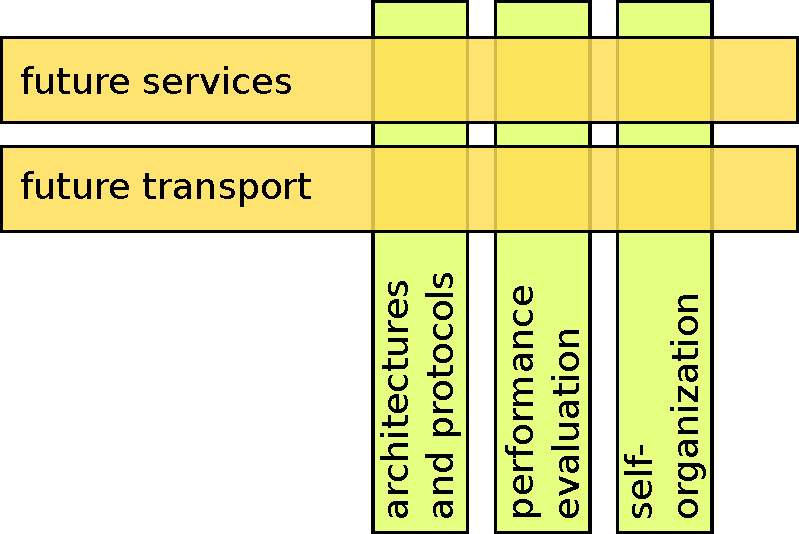
\includegraphics[width=0.7\textwidth]{images/hv-topics-new.pdf}
%     \caption{Technical solution spaces to the problem layers.}
%     \label{c1:fig:hv-topics}
% \end{figure}

%This can put pressure on the overly complex cellular network structures. The radio transmissions have only access to a limited radio frequency spectrum that, moreover, has to be shared with any other phone user in the same cell. But there is also deemed to be significant pressure on the traffic management mechanisms of the mobile core networks backing up and aggregating the numerous radio cells of an operator. 


%As discussed, the core problems are layered into services and transport. Technologically, to solve the tasks of video streaming, one can approach these  in three different ways.

%The first is to dissect the involved protocols and architectures and break them down into their functional and methodical components. This will result in an improved understanding on the manner and process of their implementation. These components serve as building blocks for generalized models that abstracts the problem space from the actual implementation. The model will be defined by a set of parameters. To explore viable parameter ranges performance evaluation methods will be facilitated.

%Secondly, using performance evaluation a system is methodically tested to the outcome of determining the influence of the system's parameters on a set of performance metrics. The parameters can be categorized into system intrinsic parameters, describing behavior only relevant and observable inside the system, and external parameters. In communication networks a good example for external parameters are the network \gls{QoS} parameters including latency, loss, jitter, and bandwidth capacity. Identifying fitting metrics for the measurement is a challenge. They can be either subjective or objective. The former are called \gls{QoE} metrics. They can only be measured by conducting empirical user studies and questionnaires and are mapped to a \gls{MOS}. Extensive work has already been done to define baseline references for QoE metrics. Using these, one can directly translate objectively measurable outcomes into \gls{QoE} metrics. However, these mappings may need to be adjusted to be able to handle stalling as the main source of quality loss. Examples for measuring subjective quality are available in \cite{gustafsson2008measuring, ketyko2010qoe}. Finally, one could employ methods of self-organization to try to reach improvements over conventional network setups.





% \begin{itemize}
%     \item ARPANAT and evolutionary process to today's Internet scale
%     \item outside and inside developments brings new Internet usage (mp3+p2p, bandwidth+codecs -> video, digicams/camcorder); socioeconomic developments of a free speech network;New traffic patterns emerging due to external developments. Digital cameras, new codecs (esp MP3, mpeg4, WebM) -> p2p, Webcams 
%     \item mobile networks: more of a parallel development to the Internet, always centralized (from the old copper/telephony/circuit switched world)
%     \item MNs very different to the Internet structures we are used to
%     \item circuit switched roots, signaling, explicitly NOT a distributed system as compared to Internet, i.e. explicit signaling central controllers
%     \item Streaming and Multicasting, Multicasting in the Internet in general (only somewhat relevant for live/realtime non-interactive stuff)
%     \item  network intelligence at the end nodes
%     \item --> end-to-end violations: ECN? only signaling, decision is e2e, same category as indirect TCP congestion control signaling (through loss) from the network; NAT, Firewalls?
%     \item content agnosticism: we do not know what applications the future will bring, so we do not make any assumptions
%     \item HTTP; ``The Web adopts relatively simple technologies with sufficient scalability efficiency and utility'' \cite{W3Arch}
%     \item Why HTTP streaming? Generalization of HTTP streaming (reliable transport, control shift to the client); Less control, more effective; Why global \gls{QoS} control doesn't work
%     \item \gls{LTE}, \gls{EPC}, Core network tunneling concepts, bottlenecks in the access and the core, \gls{LTE} network model
%     \item Improvements to congestion control for mobile streaming
%     \item Influence of L1/2/3 layer protocols and mechanisms (IPv4/6, tunneling, ethernet vs RLC/RRC/NAS, ...) ; what works better with it? compare, model and measure
%     \item \gls{QoE} metrics, \gls{MOS}, stalling time and buffering models, subjective and objective testing
%     \item http://www.ipjforum.org/?p=926 Vint Cerf looking forward

%     \item Data-mining of network trace data from mobile networks.
%     \item Investigation of mobility awareness and prediction techniques ("unassisted mobility")

%     \item Hackers: Heroes of the computer revolution \cite{levy2010hackers}
%             Computers/Hacking Culture: Build stuff first, always have running code
%     \item Baran Packet Switching
%     \item A History of the Internet and the Digital Future \cite{ryan2010history}
%             RAND
%     \item TCP/IP vint cerf + bob kahn: tcp/ip \cite{1092259}
%     \item van Jacobson Congestion Avoidance and Control \cite{jacobson1988congestion}
%     \item ISO/OSI / ATM
%     \item (Slotted) Aloha as one of the first mobile packet switched
%     \item Mobile Networks 1G/2G/3G/4G
%     \item The Web (Berners-Lee)
%     \item (Not just) A question of bandwidth Videostreaming (but also cheap access to recording devices, efficient codecs)
%     \item Camcorders

%     %% future internet stuff
%     \item HTTP as the narrow waist of the future internet \cite{Popa:2010:HNW:1868447.1868453}
%     \item The evolution of layered protocol stacks leads to an hourglass-shaped architecture \cite{akhshabi2011evolution}
%     \item The end of the end-to-end argument? \cite{reed2000endofe2e}
%     \item Where in the Internet is congestion? \cite{genin2013internet}
%     \item The Master Switch: The Rise and Fall of Information Empires \cite{wu2010master}

%     %% standard literature
%     \item Computer networking: a top-down approach \cite{kurose2008computer}
%     \item Computer networks: a systems approach \cite{peterson2007computer}

%     %% system models in general
%     \item Tracking Down Skype Traffic \cite{4509656}
%     \item The New Web: Characterizing AJAX Traffic \cite{characterizeajax2008}
%     \item Measuring Internet user traffic behavior dependent on access speed \cite{vicari1999measuring}
%     \item Measurement and modeling of WWW-sessions \cite{vicari1997measurement}
%     \item Empirically derived analytic models of wide-area TCP connections \cite{Paxson:1994:EDA:189520.189525}
%     \item Wide area traffic: the failure of Poisson modeling \cite{Paxson:1995:WAT:208389.208390}
%     \item A behavioral model of Web traffic \cite{801961}
%     \item Generating representative Web workloads for network and server performance evaluation \cite{Barford:1998:GRW:277851.277897}
%     \item Testing the IQX hypothesis for exponential interdependency between QoS and QoE of voice codecs iLBC and G. 711 \cite{hossfeld2008testing}
%     \item On the Role of Flows and Sessions in Internet Traffic Modeling: An Explorative Toy-Model \cite{5425847}
% \end{itemize}